\section{moeo\-Easy\-EA$<$ MOEOT $>$::eo\-Dummy\-Eval Class Reference}
\label{classmoeoEasyEA_1_1eoDummyEval}\index{moeoEasyEA::eoDummyEval@{moeoEasyEA::eoDummyEval}}
a dummy eval  


{\tt \#include $<$moeo\-Easy\-EA.h$>$}

Inheritance diagram for moeo\-Easy\-EA$<$ MOEOT $>$::eo\-Dummy\-Eval::\begin{figure}[H]
\begin{center}
\leavevmode
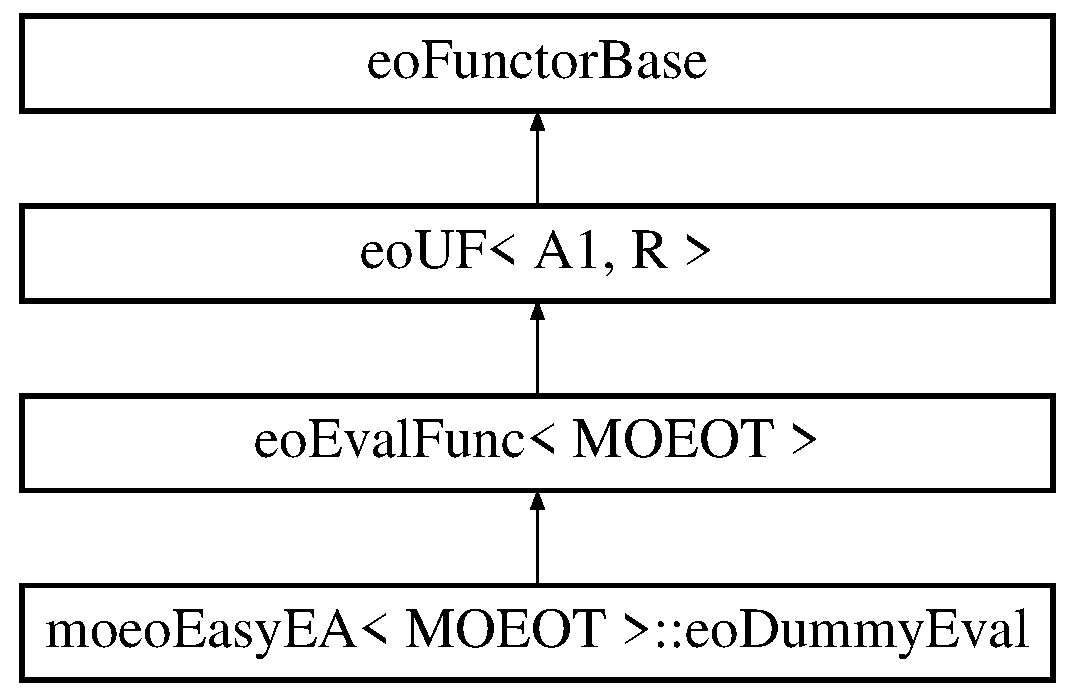
\includegraphics[height=4cm]{classmoeoEasyEA_1_1eoDummyEval}
\end{center}
\end{figure}
\subsection*{Public Member Functions}
\begin{CompactItemize}
\item 
void \bf{operator()} (MOEOT \&)\label{classmoeoEasyEA_1_1eoDummyEval_1ed55869451f883db2fc43c60f7caff5}

\begin{CompactList}\small\item\em the dummy functor \item\end{CompactList}\end{CompactItemize}


\subsection{Detailed Description}
\subsubsection*{template$<$class MOEOT$>$ class moeo\-Easy\-EA$<$ MOEOT $>$::eo\-Dummy\-Eval}

a dummy eval 



Definition at line 225 of file moeo\-Easy\-EA.h.

The documentation for this class was generated from the following file:\begin{CompactItemize}
\item 
moeo\-Easy\-EA.h\end{CompactItemize}
